\chapter{Estado del arte}

\section{SmartHome y KNX}

La \textit{smarthome} de la Universidad de Almería es un laboratorio construido con el objetivo de que tanto personal universitario como los propios alumnos pudieran investigar, trabajar y aprender sobre \textit{IoT}. La estancia está totalmente conectada a través del protocolo KNX, con el que se ha construido un ecosistema de dispositivos, sensores y actuadores con los que continuamente se realizan avances y nuevas investigaciones.

Algunos de los sensores que la componen son de temperatura, humedad, CO2 o luminosidad. Además de actuadores como los estores de las ventanas, aire acondicionado o incluso las luces. Sin embargo, no todo está conectado por KNX, sino que hay otros dispositivos conectados a la subred de la smarthome a través de TCP/HTTP por WiFi, como el altavoz Sonos, cámaras de seguridad o la Smart TV \cite{intro_4}.

\begin{figure}
    \centering
    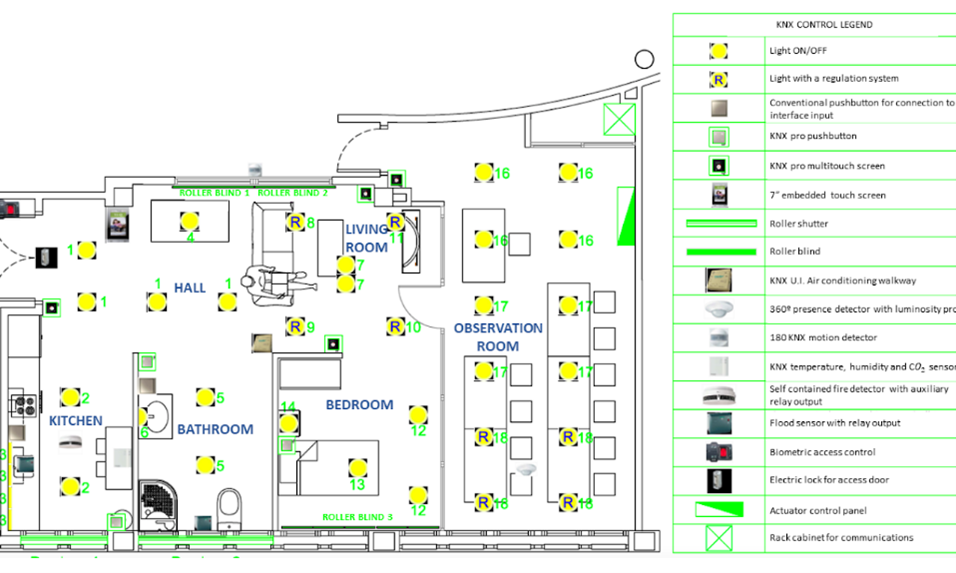
\includegraphics{imagenes/capitulo1/mapaSmarthome.png}
    \caption{Esquema de sensores y actuadores de la Smarthome}
    \label{fig:mapa_sensores}
\end{figure}

\subsection{Historia y desarrollo de KNX}

El origen de KNX es el resultado de la evolución de la domótica en las últimas décadas del siglo XX, pues se originó con la unión de tres estándares de los noventa: \textit{European Home Systems Protocol} (EHS), el \textit{European Installation Bus} (EIB) y el \textit{BatiBUS}, que pertenecían respectivamente a la \textit{European Home Systems Association} (EHSA), la \textit{European Installation Bus Association} (EIBA) y el \textit{BatiBUS Club International} (BCI).

El objetivo de esta unión era el desarrollo de un estándar común e internacional que facilitara la comunicación, gestión y compatibilidad de los dispositivos en el ámbito de la domótica. La estandarización de KNX junto con la aparición de las redes WiFi y los \textit{smartphones} proliferaron el desarrollo y el mercado de la domótica tanto a nivel industrial como doméstico durante los siguientes años \cite{intro_5}.

Gracias a esta estandarización, el control sobre la iluminación, calefacción y cualquier dispositivo KNX está es un mismo sistema, que con el paso de los años tiende a ser cada vez más automático. KNX y la domótica en sí ha ido evolucionando desde permitir controlar dispositivos a través de un panel de control o el móvil hasta no tener que controlarlo, ya que ahora mediante distintas condiciones, algoritmos e inteligencias artificiales, las decisiones y acciones se ejecutan solas.

Muchas veces, estas decisiones se toman en base a unos parámetros ideales. Por ejemplo, en este trabajo se usan parámetros atmosféricos como la temperatura o humedad, que el sistema trata de alcanzar y mantenerse. Muchas veces estos parámetros pueden ir directamente relacionados al consumo energético, de forma que se pueda controlar y limitar en todos los dispositivos, ya sea según el horario o avisando al usuario a través del móvil.

\subsection{Bases y funcionamiento de KNX}

Este protocolo parte de la idea de tener todos los dispositivos, que normalmente vamos a diferenciar entre sensores y actuadores, conectados a un “cable de comunicación” que permita intercambiar información entre ellos. Los sensores son dispositivos que detectan acciones y envían órdenes al bus en forma de telegramas. Los actuadores reciben estos telegramas y traducen las órdenes en acciones. De esta manera, un dispositivo sensor, por ejemplo, un sensor de presencia puede ordenarle a un dispositivo actuador como un relé que, siguiendo el ejemplo, encienda la luz.

\begin{figure}
    \centering
    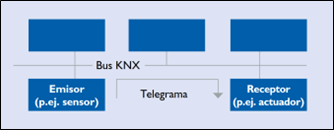
\includegraphics{imagenes/capitulo1/envioTelegrama.png}
    \caption{Envío de un telegrama por el bus KNX}
    \label{fig:envio_telegrama}
\end{figure}

Aunque la mayoría de los dispositivos se pueden englobar en sensores y actuadores, hay otros que no pueden agregarse a ninguna de estas categorías. Por ejemplo, hay muchos dispositivos con un objetivo visual, leyendo los valores de los sensores y actuadores pudiéndolo mostrar en pantallas a través de diferentes interfaces. También es común encontrar, sobre todo si la instalación es grande, un dispositivo que actúa como centro de control de toda la instalación KNX: los servidores web como SpaceLynk. Aunque más adelante hablaré algo más de este dispositivo, en resumen, permite no solo tener un control sobre todos los dispositivos conectados al bus, sino que tiene funcionalidades extras como el monitorio de la energía o el poder crear funciones lógicas que permitan codificar algoritmos que controlen los dispositivos según quiera el programador \cite{intro_6}.

Como ya he comentado, todos los dispositivos se encuentran conectados al mismo cable o bus. Esto significa que el acceso de estos al bus debe regularse y que la mayoría de los datos que se envían por el bus se utilizan para identificar a cada dispositivo que envía o reciba información. 
Este procesamiento no requiere de un dispositivo central que se encargue de dirigir los datos, sino que dicho trabajo se reparte entre todos los dispositivos del bus, ya que cada uno suele tener un microprocesador. Descentralizar la comunicación de dispositivos aporta gran autonomía al sistema, ya que, si fallara un dispositivo, no afectaría al resto de la instalación salvo a la que requiera específicamente de ese dispositivo. También aporta gran escalabilidad, aunque también depende en gran medida de la topología instalada, más adelante profundizaremos en ello.

\subsection{Medios de comunicación existentes}

Es esta sección se va a profundizar en los principales medios de comunicación existentes para KNX, principalmente en el utilizado en la Smarthome: el Par trenzado KNX.

\begin{itemize}
    \item \textbf{Par trenzado KNX (TP):} este es el medio más económico y usado, consta de un par de hilos trenzado (Twisted Pair, TP). Los dispositivos KNX se conectan al bus, que les proporciona tanto fuente de alimentación como los datos que intercambian entre ellos. La conexión se realiza a través de los denominados terminales bus, que actúan como un enchufe donde se pueden conectar tantos dispositivos como más cable de par trenzado. Este sistema aporta gran escalabilidad al sistema y seguridad, ya que aunque un dispositivo se desconecte o se rompa, el resto del sistema no se verá afectado.
    
    La forma de transmitirse los datos en de forma asíncrona, produciendo una breve bajada o subida de tensión en el caso de transmitir un 0 o un 1, respectivamente. En este medio, el telegrama es una combinación de campos que tiene diferentes objetivos:
    \begin{itemize}
        \item \textbf{Campo de control:} indica la prioridad que tiene el telegrama y si se ha repetido el envío o no.
        \item \textbf{Campo de dirección:} indica la dirección física del emisor y la del destinatario.
        \item \textbf{Campo de datos:} contiene los datos "útiles" que quiere enviar el emisor al receptor, como una orden o información.
        \item \textbf{Campo de comprobación:} indica si se ha recibido correctamente el telegrama verificando la paridad, que se comprueba enviando unos bits de paridad y un byte de comprobación. Al sumarlos todos, el resultado debe ser siempre 0.
    \end{itemize}
    \begin{figure}[h]
        \centering
        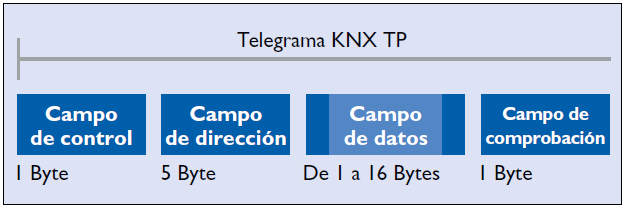
\includegraphics[width=8cm]{imagenes/capitulo2/Estructura de un telegrama KNX TP.png}
        \caption{Estructura de un telegrama KNX TP.}
        \label{fig:telegrama_KNX_TP}
    \end{figure}
    Como se ha mencionado antes, todos los dispositivos acceden al bus KNX enviando telegramas. Esto puede suponer un problema, porque si varios dispositivos envían a la vez telegramas, pueden producirse colisiones y haber pérdida de datos. Para ello se plantea un método de acceso al bus denominado CSMA/CA (Carrier Sense Multiple Access / Colission Avoidance) o de acceso aleatorio dependiendo de sucesos. Este sistema solo podrá enviar un telegrama si no hay ninguna otra transmisión en ese momento, en caso contrario se gestionarán en función de la prioridad indica en el campo de control. Si dos emisores con la misma prioridad envían a la vez datos, en el momento en el que uno que envíe un 1 se de cuenta de que otro está enviando un 0, el segundo es el que tiene la prioridad.
    
    \item \textbf{Powerline KNX (PL):} este medio aprovecha la instalación eléctrica ya existente en el edificio, no necesita un cable de bus como el KNX TP, sino que utiliza una de las tres fases y el neutro para transmitir los telegramas y aporta electricidad a los dispositivos.

    El sistema que utiliza para transmitir la información es a través del método SFSK (Spread Frequency Shift Keying), que consiste en diferencia la transmisión de un 0 o un 1 al modificar la frecuencia de la señal, 105,5 kHz para un 0 y 115,2 kHz para un 1, superponiéndose a la tensión de red.

    Gracias al aprovechamiento de la instalación eléctrica consigue ser otro medio rentable e ideal en la construcción de nuevos o rehabilitación de edificios.

    Al ser el sistema de transmisión diferente, la estructura de los telegramanas es una extensión de los del KNX PL. Se componenen de:
    \begin{itemize}
        \item \textbf{Campo de ensayo:} se utiliza para la sincronización de comunicación entre dispositivos.
        \item \textbf{Campos de preámbulo:} indican el inicio de la transmisión y gestionan el acceso al bus para tratar con las colisiones de telegramas.
        \item \textbf{Campo de contenido:} contiene el telegrama KNX con todos los campos explicados anteriormente.
        \item \textbf{Campo del ID del sistema:} indica a qué instalación KNX PL pertenece. Este campo es especialmente importante en edificios de pisos donde en una misma instalación eléctrica, pueden coexistir más de una instalación KNX.
    \end{itemize}
    \begin{figure}[h]
        \centering
        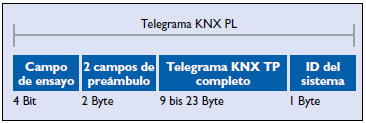
\includegraphics[width=8cm]{imagenes/capitulo2/Estructura de un telegrama KNX PL.png}
        \caption{Estructura de un telegrama KNX PL.}
        \label{fig:telegrama_KNX_PL}
    \end{figure}
    
    \item \textbf{Radiofrecuencia KNX (RF):}
    \item \textbf{KNX IP:}
\end{itemize}

\subsection{Topologías KNX más utilizadas}